\documentclass[a4paper,twocolumn]{article}
\usepackage[a4paper,left=30mm,right=30mm,top=30mm,bottom=32mm,columnsep=7.5mm]{geometry}
\usepackage{fontspec}
\setmainfont{TeX Gyre Termes}
\setsansfont{TeX Gyre Heros}
\usepackage{graphicx}
\usepackage{booktabs}
\usepackage{array}
\usepackage{xurl}
\urlstyle{same}
\usepackage[hidelinks]{hyperref}
\usepackage{microtype}
\usepackage{needspace}
\usepackage{fancyhdr}
\newfontfamily\cjkfont{HaranoAjiMincho-Regular.otf}
\renewcommand{\normalsize}{\fontsize{9pt}{11pt}\selectfont}
\setlength{\parindent}{1.5em}
\setlength{\parskip}{0pt}
\newcommand{\tablefont}{\fontsize{8pt}{10pt}\selectfont}
\renewcommand{\floatpagefraction}{0.7}
\renewcommand{\topfraction}{0.9}
\pagestyle{fancy}
\fancyhf{}
\renewcommand{\headrulewidth}{0pt}
\fancyfoot[C]{\fontsize{9pt}{11pt}\selectfont\thepage}
\fancypagestyle{plain}{\fancyhf{}\renewcommand{\headrulewidth}{0pt}\fancyfoot[C]{\fontsize{9pt}{11pt}\selectfont\thepage}}
\newcommand{\chap}[2]{\par\vspace{10pt}\needspace{4\baselineskip}\noindent{\sffamily\bfseries\fontsize{11pt}{13pt}\selectfont #1. #2\par}\vspace{4pt}\nopagebreak\noindent}
\newcommand{\chapx}[1]{\par\vspace{10pt}\needspace{4\baselineskip}\noindent{\sffamily\bfseries\fontsize{11pt}{13pt}\selectfont #1\par}\vspace{4pt}\nopagebreak\noindent}
\newcommand{\secn}[3]{\par\vspace{7pt}\needspace{3\baselineskip}\noindent{\sffamily\bfseries\fontsize{10pt}{12pt}\selectfont #1.#2 #3\par}\vspace{3pt}\nopagebreak\noindent}

\begin{document}
\twocolumn[{%
{\raggedleft\fontsize{8pt}{10pt}\selectfont SEDA GENERATIVE AI PAPERS, 2026\par}
\vspace{16pt}{\noindent\sffamily\bfseries\fontsize{10pt}{12pt}\selectfont Generative AI paper\par}
\vspace{8pt}{\noindent\sffamily\bfseries\fontsize{14pt}{18pt}\selectfont Effects of Fraction Instruction Interventions on Students' Fraction Understanding: A Meta-Analysis\par}\vspace{6pt}
{\noindent\bfseries\fontsize{11pt}{14pt}\selectfont Society for Educational Data Analysis (SEDA)\par}\vspace{8pt}
{\noindent\itshape (The Japanese version of this paper, with identical content, is available at \url{https://raw.githubusercontent.com/k518-2026/MetaAnalysisToWP/main/reports/2026-09-29-math-fraction-instruction/paper-ja.pdf}. Published September 29, 2026.)\par}\vspace{8pt}
{\noindent\fontsize{8pt}{10pt}\selectfont\textbf{\textit{Abstract}} Fractions are a persistent stumbling block in mathematics learning, and identifying instructional approaches that improve fraction understanding matters for teachers in primary and lower secondary classrooms. Using an automated workflow in which every extracted number was verified against the full text, 10 open-access studies (\textit{N} = 687) were pooled with a random-effects model. The pooled effect was \textit{g} = 0.92, 95\% CI [0.50, 1.35], with \textit{I}² = 84.5\%. These findings suggest that targeted fraction instruction can meaningfully improve fraction understanding among students in grades 1-9, though heterogeneity across studies warrants cautious interpretation.\par}\vspace{2pt}
{\noindent\fontsize{8pt}{10pt}\selectfont\textbf{\textit{Keywords}} meta-analysis, fraction instruction, mathematics education, elementary school, lower secondary school, instructional intervention\par}\vspace{10pt}
}]
\chap{1}{Introduction}
\noindent Fractions are widely recognized as one of the most conceptually demanding topics in primary and lower secondary mathematics, and difficulties with fraction understanding in these early grades are often linked to later struggles with algebra and other advanced mathematical content. Because grades 1-9 represent the period in which formal fraction instruction is introduced and consolidated, this age range is a critical window for identifying instructional practices that support robust conceptual and procedural understanding of fractions.

A wide variety of instructional interventions and teaching approaches have been designed to target fraction concepts or operations, ranging from technology-based tools to representation-based teaching sequences and error-based or language-integrated instruction. The included studies examined interventions such as dynamic digital representations [1], storytelling-based instruction [2], multiple-representations instruction [3], [4], [5], refutation texts addressing magnitude misconceptions [6], language- and mathematics-integrated scaffolding for low-achieving learners [7], gamified instruction [8], worked-out examples delivered through a web tool [9], and error-based activities [10]. These interventions were generally compared against business-as-usual instruction, an alternative teaching approach, or a no-treatment control group, with fraction knowledge or mathematics achievement tests as the outcome.

Although individual studies provide valuable evidence about specific interventions in specific contexts, the diversity of approaches, samples, and measures makes it difficult to draw general conclusions about the overall effectiveness of fraction instruction interventions from any single study. A quantitative synthesis that combines effect sizes across studies can offer a more precise and generalizable estimate of the overall effect, while also allowing exploration of variability across school levels and assessment of the robustness of the pooled result.

The purpose of this meta-analysis was therefore to synthesize the available quantitative evidence on the effects of fraction instruction interventions on students' fraction understanding in grades 1-9. Specifically, this study addressed the following research question: what is the overall effect of fraction instruction interventions on fraction understanding, and does this effect differ between elementary and middle school students?

\chap{2}{Method}
\secn{2}{1}{Literature Search}
Searches were run on September 29, 2026 in two open bibliographic sources. OpenAlex was searched in the title and abstract fields with the query “(fraction OR fractions) AND (intervention OR instruction OR teaching OR training) AND (elementary OR primary OR “middle school” OR “junior high” OR “lower secondary” OR grade OR children OR pupils)”, restricted to open-access journal articles published in 2012 or later and classified in the Education or Developmental and Educational Psychology subfields. J-STAGE, the Japanese journal platform, was searched in the abstract field with the keywords “{\cjkfont 分数} {\cjkfont 指導} {\cjkfont 小学校}”, “{\cjkfont 分数} {\cjkfont 授業} {\cjkfont 効果}” (2012 or later) to include studies published in Japan.

\secn{2}{2}{Eligibility Criteria}
Studies were eligible if they (a) sampled students in grades 1-9 (primary/elementary school and lower secondary/middle/junior high school, ages about 6-15); Exclude preschool-only, upper secondary-only, university, adult, and teacher/pre-service teacher samples; (b) examined an instructional intervention or teaching approach targeting fraction concepts or operations; (c) compared it with business-as-usual instruction, an alternative instruction, or a no-treatment control group; (d) measured a fraction knowledge test or mathematics achievement test; and (e) reported statistics sufficient to compute a standardized mean difference. Reviews, qualitative studies, single-case designs, and single-group pre-post designs were excluded.

\secn{2}{3}{Screening and Data Extraction}
Screening and data extraction were automated. A large language model (claude-sonnet-5) rated each title and abstract against the eligibility criteria. Full texts (PDF) of the highest-rated records were retrieved and converted to plain text, and the model extracted study characteristics and summary statistics from them. Every extracted number was then checked by software against the full text, and a study was excluded from the synthesis if any extracted number could not be found verbatim. No human reviewer verified the screening or the extraction. When more than 10 studies qualified, the 10 with the highest screening ratings were retained.

\secn{2}{4}{Effect Sizes}
Standardized mean differences were computed as Hedges’ g [11] from post-test means, standard deviations, and group sizes; when these were unavailable, from independent-samples t statistics, from F statistics with one numerator degree of freedom, or from reported d or g values. Positive values indicate higher scores in the intervention group. One effect size per study was used.

\secn{2}{5}{Statistical Analysis}
Effect sizes were pooled with a random-effects model in which the between-study variance (\textit{τ}²) was estimated with the DerSimonian–Laird method [12]. Confidence intervals and tests of the pooled effect used the Hartung–Knapp–Sidik–Jonkman (HKSJ) adjustment, which is recommended when the number of studies is small [13], [14]. Heterogeneity was assessed with Q, \textit{I}² [15], \textit{τ}², and a 95\% prediction interval. Subgroup analyses by school level (elementary: grades 1–6; lower secondary: grades 7–9) were conducted when each level included at least two studies. Robustness was examined with leave-one-out analysis, and Egger’s regression test [16] was planned only when at least 10 studies were available. Effect magnitudes were interpreted with conventional benchmarks [17]. Analyses followed standard formulas [18] implemented in open-source JavaScript code (\url{https://github.com/k518-2026/MetaAnalysisToWP}).

\chap{3}{Results}
\secn{3}{1}{Study Selection}
The searches returned 150 records from OpenAlex (of 331 matching the query) and 5 from J-STAGE, for 154 unique records. Of the 145 records with abstracts that were screened, 31 were rated as potentially eligible. Full texts of 26 records were examined: 11 could not be retrieved or read, 0 did not meet the eligibility criteria, 2 did not report sufficient statistics, 3 contained extracted numbers that could not be verified in the text, and 0 yielded implausible values. In total, 10 studies were included in the meta-analysis.

\secn{3}{2}{Study Characteristics}
Table 1 summarizes the country, grade, design, sample size, and effect size of each included study [1], [2], [3], [4], [5], [6], [7], [8], [9], [10]. The studies comprised 687 participants in total and were conducted in Turkey, Greece, Ghana, Belgium, Germany, South Africa, India. By school level, 8 studies sampled elementary (grades 1–6) students, 2 studies sampled lower secondary (grades 7–9) students. Sample sizes ranged from 40 to 120, and individual effect sizes ranged from \textit{g} = \ensuremath{-}0.25 to \textit{g} = 1.96.

\begin{table*}[tb]
\centering
{\tablefont \textbf{Table 1.} Overview of the Included Studies\par}\vspace{2pt}
{\tablefont\renewcommand{\arraystretch}{1.12}
\begin{tabular}{>{\raggedright\arraybackslash}p{0.2600\dimexpr\textwidth-12\tabcolsep\relax}>{\raggedright\arraybackslash}p{0.1100\dimexpr\textwidth-12\tabcolsep\relax}>{\raggedright\arraybackslash}p{0.1200\dimexpr\textwidth-12\tabcolsep\relax}>{\raggedright\arraybackslash}p{0.2300\dimexpr\textwidth-12\tabcolsep\relax}>{\raggedright\arraybackslash}p{0.0700\dimexpr\textwidth-12\tabcolsep\relax}>{\raggedright\arraybackslash}p{0.2100\dimexpr\textwidth-12\tabcolsep\relax}}
\toprule
Study & Country & Grade & Design & \textit{N} & \textit{g} [95\% CI] \\
\midrule
Bulut et al. [1] & Turkey & Grade 3 & quasi-experimental & 40 & 0.83 [0.20, 1.47] \\
Lemonidis and Kaiafa [2] & Greece & Grade 3 & quasi-experimental & 76 & 0.57 [0.12, 1.03] \\
Mahama and Kyeremeh [3] & Ghana & Grade 6 & quasi-experimental (non-equivalent control group design) & 96 & 1.39 [0.94, 1.83] \\
Van Hoof et al. [6] & Belgium & Grade 4 & randomized controlled trial & 76 & \ensuremath{-}0.25 [\ensuremath{-}0.69, 0.20] \\
Prediger and Wessel [7] & Germany & Grade 7 & quasi-experimental pre-test post-test control group design with random assignment to matched pairs & 72 & 0.86 [0.38, 1.34] \\
Ubah [4] & South Africa & Grade 5 & quasi-experimental (nonequivalent control group, pre-test/post-test) & 120 & 1.96 [1.53, 2.40] \\
Pal [5] & India & Grade 4 & quasi-experimental & 40 & 1.28 [0.61, 1.95] \\
KARAMERT and Vardar [8] & Turkey & Grade 5 & quasi-experimental & 46 & 0.65 [0.07, 1.24] \\
Tahiroğlu and Özcan [9] & Turkey & Grade 5 & quasi-experimental & 77 & 1.15 [0.67, 1.63] \\
Sancar and Özkaya [10] & Turkey & Grade 6 & quasi-experimental & 44 & 0.77 [0.16, 1.37] \\
\bottomrule
\end{tabular}\par}
\vspace{2pt}{\tablefont\noindent \textit{Note.} CI = confidence interval. \textit{g} = Hedges’ g (positive values favor the intervention). Grades and designs were extracted automatically from the full texts.\par}
\end{table*}
Table 2 lists the intervention, comparison condition, and outcome measure of each study. All 10 studies compared an intervention group with a comparison group on a post-test.

\begin{table*}[tb]
\centering
{\tablefont \textbf{Table 2.} Interventions, Comparison Conditions, and Outcome Measures\par}\vspace{2pt}
{\tablefont\renewcommand{\arraystretch}{1.12}
\begin{tabular}{>{\raggedright\arraybackslash}p{0.2000\dimexpr\textwidth-8\tabcolsep\relax}>{\raggedright\arraybackslash}p{0.3200\dimexpr\textwidth-8\tabcolsep\relax}>{\raggedright\arraybackslash}p{0.2400\dimexpr\textwidth-8\tabcolsep\relax}>{\raggedright\arraybackslash}p{0.2400\dimexpr\textwidth-8\tabcolsep\relax}}
\toprule
Study & Intervention & Comparison & Outcome \\
\midrule
Bulut et al. [1] & GeoGebra dynamic representational activities for teaching fractions & Traditional/normal fraction teaching sequence & 22-item fractions academic achievement post-test (48 sub-questions) \\
Lemonidis and Kaiafa [2] & Teaching fractions using target-focused storytelling with picture stories & Teaching fractions using manipulative materials (objects, area models, number lines) & 10-item fraction achievement post-test \\
Mahama and Kyeremeh [3] & Multiple representations-based instruction (paper folding, number line, symbols, verbal) & Conventional lecture/discussion instruction on common fractions & 10-item common fraction problem-solving test (post-test, out of 30) \\
Van Hoof et al. [6] & Refutation text explicitly refuting fraction magnitude misconception & Expository text explaining fractions without addressing misconception & Accuracy on computerized fraction magnitude comparison test \\
Prediger and Wessel [7] & Language- and mathematics-integrated intervention relating registers, pushed output, and scaffolding for fractions & Regular classroom instruction with usual fraction textbook repetition program & Standardised fraction test (41 items) post-test score \\
Ubah [4] & Teacher Ben's approach using multiple representations (concrete-to-semi-concrete-to-symbolic) and learner-centered activities for addition of fractions & Teacher Will's approach using teacher-led demonstrations with limited representation connections & Fraction Achievement Test (FAT) post-test score on addition of fractions \\
Pal [5] & Multiple representations based instructional program using manipulatives, pictures, and problem solving for fractions & Conventional/traditional fraction instruction taught discretely without connecting representations & Fraction concepts test (pre-test and post-test scores) \\
KARAMERT and Vardar [8] & Gamified fraction instruction using Pyramidal Design Model elements (progress map, badges, avatars) & Standard non-gamified fraction instruction following the same curriculum & Teacher-developed 24-item academic achievement test on fractions \\
Tahiroğlu and Özcan [9] & Worked-out examples with multiple solution methods delivered via Nearpod Web 2.0 tool & Textbook-based activities delivered via Nearpod with single solution method & Fraction Achievement Test (FAT) post-test score \\
Sancar and Özkaya [10] & Error-based activity (EBA) fraction instruction using incorrect and correct solutions with discussion & Standard mathematics curriculum instruction without error-based activities & Subject Comprehension Test (SCT) fraction achievement post-test \\
\bottomrule
\end{tabular}\par}
\vspace{2pt}{\tablefont\noindent \textit{Note.} Extracted and summarized automatically from the full texts.\par}
\end{table*}
\secn{3}{3}{Overall Effect}
Fig. 1 shows the forest plot. Each square marks the effect size of one study, with its size proportional to the study’s weight, and each horizontal line marks the 95\% confidence interval; the diamond at the bottom is the pooled estimate. 9 of the 10 studies had positive effect sizes, and the confidence intervals of 9 studies did not include zero. The study with the largest weight was Ubah [4] (10.5\%).

\begin{figure*}[tb]
\centering
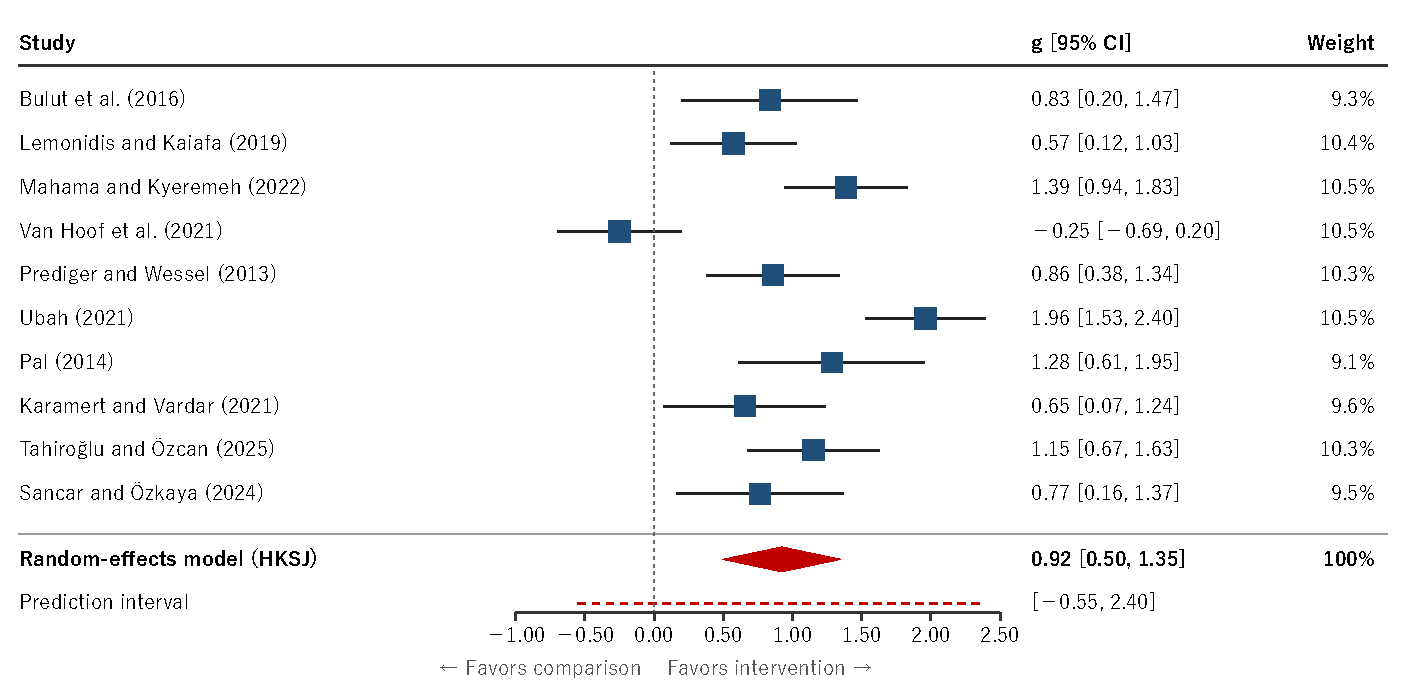
\includegraphics[width=\textwidth]{forest-en.pdf}\par\vspace{2pt}
{\tablefont\textbf{Figure 1.} Forest plot of individual and pooled effect sizes\par}{\tablefont Squares show study effect sizes (size proportional to weight), lines show 95\% confidence intervals, the diamond shows the pooled estimate, and the dashed line shows the prediction interval.\par}
\end{figure*}
The random-effects model yielded a pooled effect of \textit{g} = 0.92, 95\% CI [0.50, 1.35], \textit{t}(9) = 4.89, p < .001, which corresponds to a large effect by conventional benchmarks. The fixed-effect estimate was \textit{g} = 0.93. Table 3 summarizes these estimates.

\secn{3}{4}{Heterogeneity}
Heterogeneity was considerable, \textit{Q}(9) = 58.14, p < .001, \textit{I}² = 84.5\%, \textit{τ}² = 0.364. The 95\% prediction interval ranged from \ensuremath{-}0.55 to 2.40.

\secn{3}{5}{Subgroup and Sensitivity Analyses}
For elementary (grades 1–6) samples, \textit{g} = 0.95, 95\% CI [0.39, 1.51] (\textit{k} = 8); for lower secondary (grades 7–9) samples, \textit{g} = 0.82, 95\% CI [0.24, 1.40] (\textit{k} = 2). The difference between school levels was not statistically significant, \textit{Q}(1) = 0.28, \textit{p} = .598. Leave-one-out estimates ranged from 0.80 to 1.07. Egger’s test did not indicate funnel plot asymmetry (intercept = \ensuremath{-}1.13, \textit{p} = .846). The subgroup estimates are also shown in Table 3.

\begin{table*}[tb]
\centering
{\tablefont \textbf{Table 3.} Results of the Meta-Analysis\par}\vspace{2pt}
{\tablefont\renewcommand{\arraystretch}{1.12}
\begin{tabular}{lrrrrrrr}
\toprule
Model & \textit{k} & \textit{N} & \textit{g} & 95\% CI & \textit{p} & \textit{I}² (\%) & \textit{τ}² \\
\midrule
Random effects (HKSJ) & 10 & 687 & 0.92 & [0.50, 1.35] & < .001 & 84.5 & 0.364 \\
Fixed effect & 10 & 687 & 0.93 & [0.77, 1.09] & < .001 & — & — \\
\hspace{1em}elementary (grades 1–6) & 8 & 571 & 0.95 & [0.39, 1.51] & .005 & 87.9 & 0.473 \\
\hspace{1em}lower secondary (grades 7–9) & 2 & 116 & 0.82 & [0.24, 1.40] & .035 & 0.0 & 0.000 \\
\bottomrule
\end{tabular}\par}
\vspace{2pt}{\tablefont\noindent \textit{Note.} \textit{k} = number of studies. HKSJ = Hartung–Knapp–Sidik–Jonkman confidence interval. 95\% prediction interval [\ensuremath{-}0.55, 2.40].\par}
\end{table*}
\chap{4}{Discussion}
The pooled effect across the ten included studies indicated a large positive effect of fraction instruction interventions on students' fraction understanding, suggesting that, on average, students receiving these targeted interventions substantially outperformed students in comparison conditions on fraction knowledge or mathematics achievement measures. This magnitude of effect is considerably larger than what is typically observed for general educational interventions, suggesting that well-designed fraction-specific instruction may offer meaningful benefits over business-as-usual or alternative teaching approaches.

However, the heterogeneity statistics indicate substantial variability in effect sizes across studies, with a wide prediction interval that even includes negative values. This suggests that although the average effect is strongly positive, the effect of a given intervention in a new, similar context could plausibly range from null or even slightly negative to very large. This variability likely reflects genuine differences among the interventions studied, which ranged from technology-based tools [1], [9] to representation-based teaching [3], [4], [5], language-integrated scaffolding for low-achieving learners [7], gamification [8], and error-based instruction [10], as well as differences in comparison conditions, outcome measures, and sample characteristics.

The subgroup analysis comparing elementary and middle school levels showed similar effect sizes for both groups, and the test for subgroup differences was not statistically significant, indicating that the benefits of fraction instruction interventions may generalize across this range of grade levels rather than being specific to either primary or lower secondary education. The leave-one-out sensitivity analysis showed that the pooled estimate remained consistently large and positive across all iterations, suggesting that no single study disproportionately drove the overall result, which lends some confidence to the robustness of the general pattern despite the observed heterogeneity.

Notably, one included study [6], which examined a refutation text intervention targeting a specific fraction magnitude misconception, found a small negative effect favoring the comparison condition, in contrast to the generally strong positive effects observed in studies using representation-based or activity-based instructional approaches [3], [4], [5], [9]. This contrast suggests that not all forms of fraction-related instruction are equally effective, and that interventions involving active, representation-rich, or error-focused engagement with fraction concepts may be particularly promising.

For teachers in grades 1-9, these findings tentatively suggest that incorporating multiple representations, active problem-solving, technology-supported tools, or targeted scaffolding into fraction instruction may support stronger student understanding than conventional teaching alone. However, given the variability across studies, teachers and school leaders should consider the specific instructional approach and context rather than assuming uniform benefits from any single method.

\chap{5}{Conclusion}
This meta-analysis of ten studies found a large, statistically significant overall effect of fraction instruction interventions on students' fraction understanding in grades 1-9, with no significant difference between elementary and middle school levels and a robust result across sensitivity analyses. However, substantial heterogeneity among studies and the small number of included studies indicate that these findings should be interpreted as an encouraging but preliminary synthesis, highlighting the need for further high-quality research to clarify which specific instructional features most reliably support fraction understanding across primary and lower secondary education.

This meta-analysis is based on a small number of studies (\textit{k} = 10), which limits the precision and generalizability of the pooled estimate and constrains the statistical power of subgroup and sensitivity analyses, particularly the comparison between elementary and middle school levels, which included only two studies at the middle school level. The small number of studies also means that the pooled effect and heterogeneity estimates should be interpreted with caution, as they may be sensitive to the addition of future studies.

Additionally, the included studies relied predominantly on quasi-experimental designs with only one randomized controlled trial, used varied and often researcher-developed outcome measures, and drew on samples from a limited set of countries, which may affect the comparability and generalizability of the pooled results. Effect sizes and study characteristics were extracted automatically, which may introduce inaccuracies not fully captured in this synthesis.

In addition, screening and data extraction were automated with a language model, and extracted numbers were verified only by matching them against the full text. A number can be present in the text yet belong to a different group or measure. Only open-access studies whose full texts could be retrieved were included; subscription-only and unpublished studies were not.

\chapx{Author notes}
This is a “Generative AI paper” produced automatically by the Society for Educational Data Analysis (SEDA) with generative AI. Large language models (claude-sonnet-5) were used to screen records, extract data, and draft the Introduction, Discussion, and Conclusion; all statistics were computed by software. The paper has not been peer reviewed.

Data and code are available at \url{https://github.com/k518-2026/MetaAnalysisToWP}. © 2026 Society for Educational Data Analysis (SEDA).

\chapx{References}
\noindent References marked with an asterisk indicate studies included in the meta-analysis.\par
{\fontsize{8.5pt}{10.5pt}\selectfont
\par\noindent\hangindent=2.4em\hangafter=1 \makebox[2.4em][l]{[1]}*M. Bulut, H. Ü. Akçakın, G. Kaya, and V. Akçakın, “The Effects of GeoGebra On Third Grade Primary Students’ Academic Achievement in Fractions,” \textit{International Electronic Journal of Mathematics Education}, vol. 11, no. 2, pp. 347–255, 2016, doi: 10.29333/iejme/338.\par
\par\noindent\hangindent=2.4em\hangafter=1 \makebox[2.4em][l]{[2]}*C. Lemonidis and I. Kaiafa, “The Effect of Using Storytelling Strategy on Students’ Performance in Fractions,” \textit{Journal of Education and Learning}, vol. 8, no. 2, p. 165, 2019, doi: 10.5539/jel.v8n2p165.\par
\par\noindent\hangindent=2.4em\hangafter=1 \makebox[2.4em][l]{[3]}*P. N. Mahama and P. Kyeremeh, “Impact of multiple representations-based instruction on basic six pupils’ performance in solving problems on common fractions,” \textit{Journal of Mathematics and Science Teacher}, vol. 3, no. 1, p. em023, 2022, doi: 10.29333/mathsciteacher/12610.\par
\par\noindent\hangindent=2.4em\hangafter=1 \makebox[2.4em][l]{[4]}*I. J. Ubah, “The impact of different approaches to the teaching of Grade 5 fraction by three experienced teachers,” \textit{South African Journal of Childhood Education}, vol. 11, no. 1, 2021, doi: 10.4102/sajce.v11i1.854.\par
\par\noindent\hangindent=2.4em\hangafter=1 \makebox[2.4em][l]{[5]}*M. Pal, “Making Conceptual Knowledge Connections to Clear Misconceptions in Fractions in Primary Classrooms,” \textit{IOSR Journal of Research \& Method in Education (IOSRJRME)}, vol. 4, no. 2, pp. 12–18, 2014, doi: 10.9790/7388-04241218.\par
\par\noindent\hangindent=2.4em\hangafter=1 \makebox[2.4em][l]{[6]}*J. Van Hoof, A.-S. Engelen, and W. Van Dooren, “How robust are learners’ misconceptions of fraction magnitude? An intervention study comparing the use of refutation and expository text,” \textit{Educational Psychology}, vol. 41, no. 5, pp. 524–543, 2021, doi: 10.1080/01443410.2021.1908521.\par
\par\noindent\hangindent=2.4em\hangafter=1 \makebox[2.4em][l]{[7]}*S. Prediger and L. Wessel, “Fostering German-language learners’ constructions of meanings for fractions—design and effects of a language- and mathematics-integrated intervention,” \textit{Mathematics Education Research Journal}, vol. 25, no. 3, pp. 435–456, 2013, doi: 10.1007/s13394-013-0079-2.\par
\par\noindent\hangindent=2.4em\hangafter=1 \makebox[2.4em][l]{[8]}*Ö. KARAMERT and A. K. Vardar, “The effect of gamification on young mathematics learners’ achievements and attitudes,” \textit{Journal of Educational Technology and Online Learning}, vol. 4, no. 2, pp. 96–114, 2021, doi: 10.31681/jetol.904704.\par
\par\noindent\hangindent=2.4em\hangafter=1 \makebox[2.4em][l]{[9]}*N. G. Tahiroğlu and Z. Ç. Özcan, “Impact of worked-out examples via a Web 2.0 tool on fifth graders achievement, attitudes, and motivation in mathematics,” \textit{Journal of Pedagogical Research}, 2025, doi: 10.33902/jpr.202533896.\par
\par\noindent\hangindent=2.4em\hangafter=1 \makebox[2.4em][l]{[10]}*E. Sancar and M. Özkaya, “Error-based Activity Applications in Sixth Grade Fraction Teaching,” \textit{Studia paedagogica}, vol. 29, no. 2, pp. 33–65, 2024, doi: 10.5817/sp2024-2-2.\par
\par\noindent\hangindent=2.4em\hangafter=1 \makebox[2.4em][l]{[11]}L. V. Hedges, “Distribution theory for Glass's estimator of effect size and related estimators,” \textit{Journal of Educational Statistics}, vol. 6, no. 2, pp. 107–128, 1981, doi: 10.3102/10769986006002107.\par
\par\noindent\hangindent=2.4em\hangafter=1 \makebox[2.4em][l]{[12]}R. DerSimonian and N. Laird, “Meta-analysis in clinical trials,” \textit{Controlled Clinical Trials}, vol. 7, no. 3, pp. 177–188, 1986, doi: 10.1016/0197-2456(86)90046-2.\par
\par\noindent\hangindent=2.4em\hangafter=1 \makebox[2.4em][l]{[13]}J. Hartung and G. Knapp, “A refined method for the meta-analysis of controlled clinical trials with binary outcome,” \textit{Statistics in Medicine}, vol. 20, no. 24, pp. 3875–3889, 2001, doi: 10.1002/sim.1009.\par
\par\noindent\hangindent=2.4em\hangafter=1 \makebox[2.4em][l]{[14]}J. IntHout, J. P. A. Ioannidis, and G. F. Borm, “The Hartung-Knapp-Sidik-Jonkman method for random effects meta-analysis is straightforward and considerably outperforms the standard DerSimonian-Laird method,” \textit{BMC Medical Research Methodology}, vol. 14, Art. no. 25, 2014, doi: 10.1186/1471-2288-14-25.\par
\par\noindent\hangindent=2.4em\hangafter=1 \makebox[2.4em][l]{[15]}J. P. T. Higgins and S. G. Thompson, “Quantifying heterogeneity in a meta-analysis,” \textit{Statistics in Medicine}, vol. 21, no. 11, pp. 1539–1558, 2002, doi: 10.1002/sim.1186.\par
\par\noindent\hangindent=2.4em\hangafter=1 \makebox[2.4em][l]{[16]}M. Egger, G. Davey Smith, M. Schneider, and C. Minder, “Bias in meta-analysis detected by a simple, graphical test,” \textit{BMJ}, vol. 315, no. 7109, pp. 629–634, 1997, doi: 10.1136/bmj.315.7109.629.\par
\par\noindent\hangindent=2.4em\hangafter=1 \makebox[2.4em][l]{[17]}J. Cohen, \textit{Statistical Power Analysis for the Behavioral Sciences}, 2nd ed. Lawrence Erlbaum Associates, 1988.\par
\par\noindent\hangindent=2.4em\hangafter=1 \makebox[2.4em][l]{[18]}M. Borenstein, L. V. Hedges, J. P. T. Higgins, and H. R. Rothstein, \textit{Introduction to Meta-Analysis}, Wiley, 2009, doi: 10.1002/9780470743386.\par
}
\end{document}
